\documentclass{EESD}
% To change the slides size go to EESD.cls file and edit the preamble as explained.

% ---- Add your Meta-data to the PDF (Copyrights Kinda!) ----
\hypersetup{
  pdfinfo={
    Title={Presentation: 3D finite element modeling of historical masonry walls},
    Author={Mahmoud S. Shaqfa, Katrin Beyer},
    Subject={EPFL - ENAC - EESD Lab},
    Keywords={Stone masonry, Detailed micro-mechanical, 3D micro-structure}
  }
}

% Important packages to be called
\usepackage{subcaption} % for adding sub-figures
\usepackage{graphicx}
\usepackage[absolute,overlay]{textpos} % To place the figures by coordinates (x,y) - Beamer doesn't support floats XD
\usepackage{multicol} % To adjust items and stuff automatically in a number of a pre-specified columns
\graphicspath{{Figures/}}
\usepackage[utf8]{inputenc}
\usepackage{amsmath}
\usepackage{amsfonts}
\usepackage{amssymb}
\usepackage{lipsum} % Just a dummy text generator
\usepackage{hyperref}
% fonts packages
\usepackage{ragged2e} % Justified typesetting

% For References Only
\usepackage[style=authortitle,backend=bibtex]{biblatex}
\addbibresource{References.bib} % Call the references database
\AtBeginBibliography{\tiny} % Specify font size (Size matters)
\renewcommand{\footnotesize}{\tiny}

% For adding code blocks
\usepackage{listings}
\lstset
{
    language=[LaTeX]TeX,
    breaklines=true,
    basicstyle=\tt\scriptsize,
    keywordstyle=\color{blue},
    identifierstyle=\color{magenta},
    commentstyle=\color{red},
    rulecolor=\color{black},
    numbers=left,
    numberstyle=\tiny\color{black},
    % framexleftmargin=15pt,
    frame = single,
}


\author{The Templater}
\title[Your tiny title here]{My long, detailed, and flashy title}

\institute[ENAC]{{\'Ecole Polytechnique F\'ed\'erale de Lausanne (EPFL)}{\newline\newline School of Architecture, Civil and Environmental Engineering (ENAC)}}
\subject{Candidacy Exam}
\date{May 2019}

\begin{document}

% To define the cover-page here .. I prefer this
{
\usebackgroundtemplate{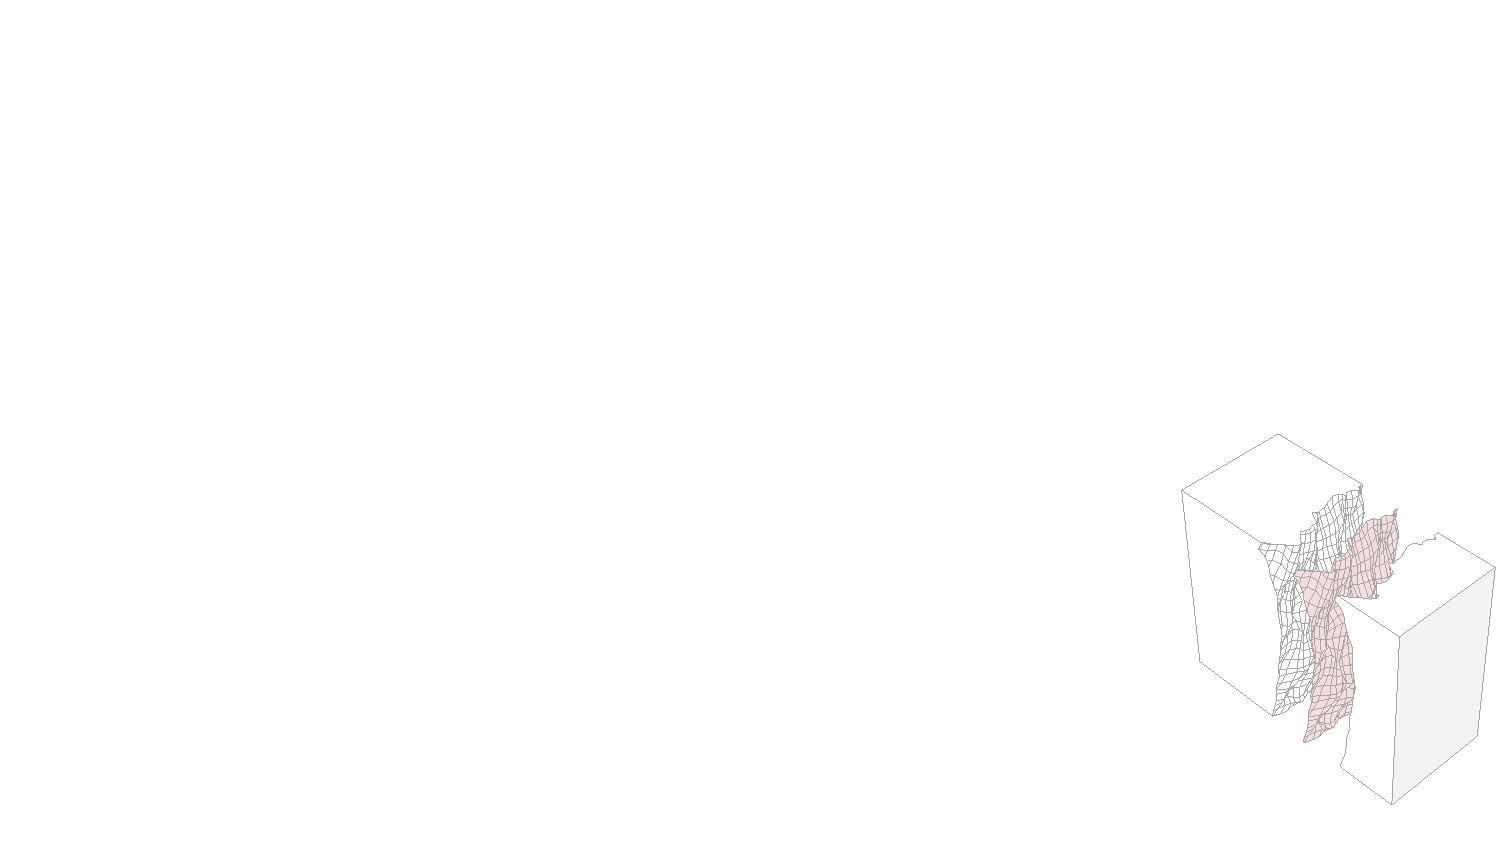
\includegraphics[width=1.\paperwidth, height=1.\paperheight]{cover169.pdf}} % To add a background for this slide XD - change it
\coverpage{
\titlepage{~}
% To add additional text to the title components 
{\newline Supervisor: Prof. Katrin Beyer}
}
}

\setbeamertemplate{logo}{} % To override the logo from the other slides and delete it completely


% -----------------------Table of contents TOC Three Styles
% Explicitly split the TOC if it's too long
% \begin{frame}[allowframebreaks]{Outlines}
% \tableofcontents[sections={1-3}] % Explicitly split TOC
% \framebreak
% \tableofcontents[sections={4-7}] % Explicitly split TOC
% \end{frame}

% % Just a normal TOC 
% \begin{frame}[allowframebreaks]{Outlines}
% \tableofcontents
% \end{frame}

% Use smart division for the TOC
\begin{frame}{Outlines}
\begin{multicols}{2}
\tableofcontents
\end{multicols}
\end{frame}

% -----------------------Introduction
\section{Introduction}

\breakingframe{
\begin{textblock*}{3cm}[0.5,0.5](0.5\textwidth,  0.5\textheight)
\Huge\textbf{\textcolor{black}{Introduction}}
\end{textblock*}
}

\subsection{Copyright}
\begin{frame}[t]{Copyright}
\begin{textblock*}{13cm}(1.0cm,  1.7cm)
    {\fontfamily{qcr}\selectfont
    This file is a customized "beamer" template made for the EESD laboratory at EPFL (see \href{https://www.epfl.ch/labs/eesd/}{https://www.epfl.ch/labs/eesd/}). The author of this file is \textbf{Mahmoud S. Shaqfa}. This file is free: you can redistribute it and/or modify it under the terms of the GNU General Public License as published by    the Free Software Foundation, either version 3 of the License, or (at your option) any later version. This file is distributed in the hope that it will be useful, but WITHOUT ANY WARRANTY; without even the implied warranty of MERCHANTABILITY or FITNESS FOR A PARTICULAR PURPOSE.  See the GNU General Public License for more details. To receive a copy of GNU License refer to: \href{https://www.gnu.org/licenses/}{https://www.gnu.org/licenses/}
    }
\end{textblock*}
\end{frame}

\subsection{Cover page}
\begin{frame}[fragile]
\frametitle{Cover page}
    To define the cover page use the following code:
    \vspace{10pt}
    \begin{lstlisting}
    { % <-- Important to add those brackets; to affect only the background in this frame.
    \usebackgroundtemplate{\includegraphics[]{}} % <-- Define the background here
        \coverpage{
            \titlepage % make the title here
            {\newline Additional text like the supervisors, jury .. etc}
        }
        }
    } % <-- end of the environment
    \end{lstlisting}
    \texttt{\small{\textcolor{red}{\textbf{A dummy note}}: to define a very good background you can create a PDF file of the slide size and place it with any graphical effects by using Inkscape or Illustrator (see ../Figures/cover169.pdf or ../Figures/cover43.pdf).}}
    \vspace{10pt}
\end{frame}

\subsection{Table of contents (TOC)}
\begin{frame}[fragile]
\frametitle{TOC options}
    \vspace{5pt}
    \begin{lstlisting}
        \tableofcontents % <-- Traditional TOC
    \end{lstlisting}
    \vspace{5pt}
    \begin{lstlisting}
        \tableofcontents[sections={1-3}] % <-- Explicitly split TOC
    \end{lstlisting}
    \vspace{5pt}
    \begin{lstlisting}
    \usepackage{multicol}
    \begin{multicols}{2} % <-- Smart division (2, 3, ..etc any number of columns)
        \tableofcontents
    \end{multicols}
    \end{lstlisting}
    \vspace{5pt}
    And define the frame to automatically divide itself when the TOC is too long to fit in a single frame:
    \begin{lstlisting}
    % \begin{frame}[allowframebreaks]{Table of contents}
    % \end{frame}
    \end{lstlisting}
\end{frame}

\section{How to use?}
\breakingframe{
    \begin{textblock*}{5cm}[0.3,0.5](0.5\textwidth, 0.5\textheight)
        \textbf{\Huge{How to use?}}
    \end{textblock*}
}

\subsection{Beamer blocks}
\begin{frame}[fragile]
\frametitle{How to use blocks?}
    Basically, the blocks style have been modified in "beamer" in this customized version. Programmatic samples can be found in the next three slides.
    \vspace{10pt}
    \begin{lstlisting}
        \begin{block}{The block title}
            The block body .. add meaningful stuff
        \end{block}
    \end{lstlisting}
    \vspace{10pt}
    It can be used for definitions, equations, theories, examples, alerts, and important stuff to highlight.
\end{frame}

\begin{frame}
\frametitle{Blocky block}
\begin{block}{Just a Block}
\lipsum[1]
\end{block}
\end{frame}

\begin{frame}
\frametitle{Blocky block}
\begin{exampleblock}{Example Block}
\lipsum[1]
\end{exampleblock}
\end{frame}

\begin{frame}
\frametitle{Blocky block}
\begin{alertblock}{Alert Block}
\lipsum[1]
\end{alertblock}
\end{frame}

\subsection{Frames breaker}
\begin{frame}[fragile]
\frametitle{How to use frame-breakings?}
    In this template, and only this, I defined a "breakingframe" template frame that should not hold any useful information. The background of this frame is pinkish solid and it is not countable as a separate frame. You can use this as a transitioning page between different topics or for any funny funky stuff to release the tense of the poor audience during your presentation.
    \vspace{10pt}
    \begin{lstlisting}
        \breakingframe{
            Put your contents here, such as images, text ..etc. Be as silly as possible .. or not!
        }
    \end{lstlisting}
    \vspace{10pt}
    Look at the next slide, in code, as an example!
\end{frame}

\breakingframe{
    \begin{textblock*}{10cm}[0.40,0.5](0.55\textwidth, 0.5\textheight)
        \textbf{\Huge{I'm just an example!}}
    \end{textblock*}
    
    \begin{textblock*}{7cm}[0.40,0.5](0.4\textwidth, 0.8\textheight)
        
\includegraphics[height = 0.3\textheight]{cat.jpeg}
    \end{textblock*}
}

{
\usebackgroundtemplate{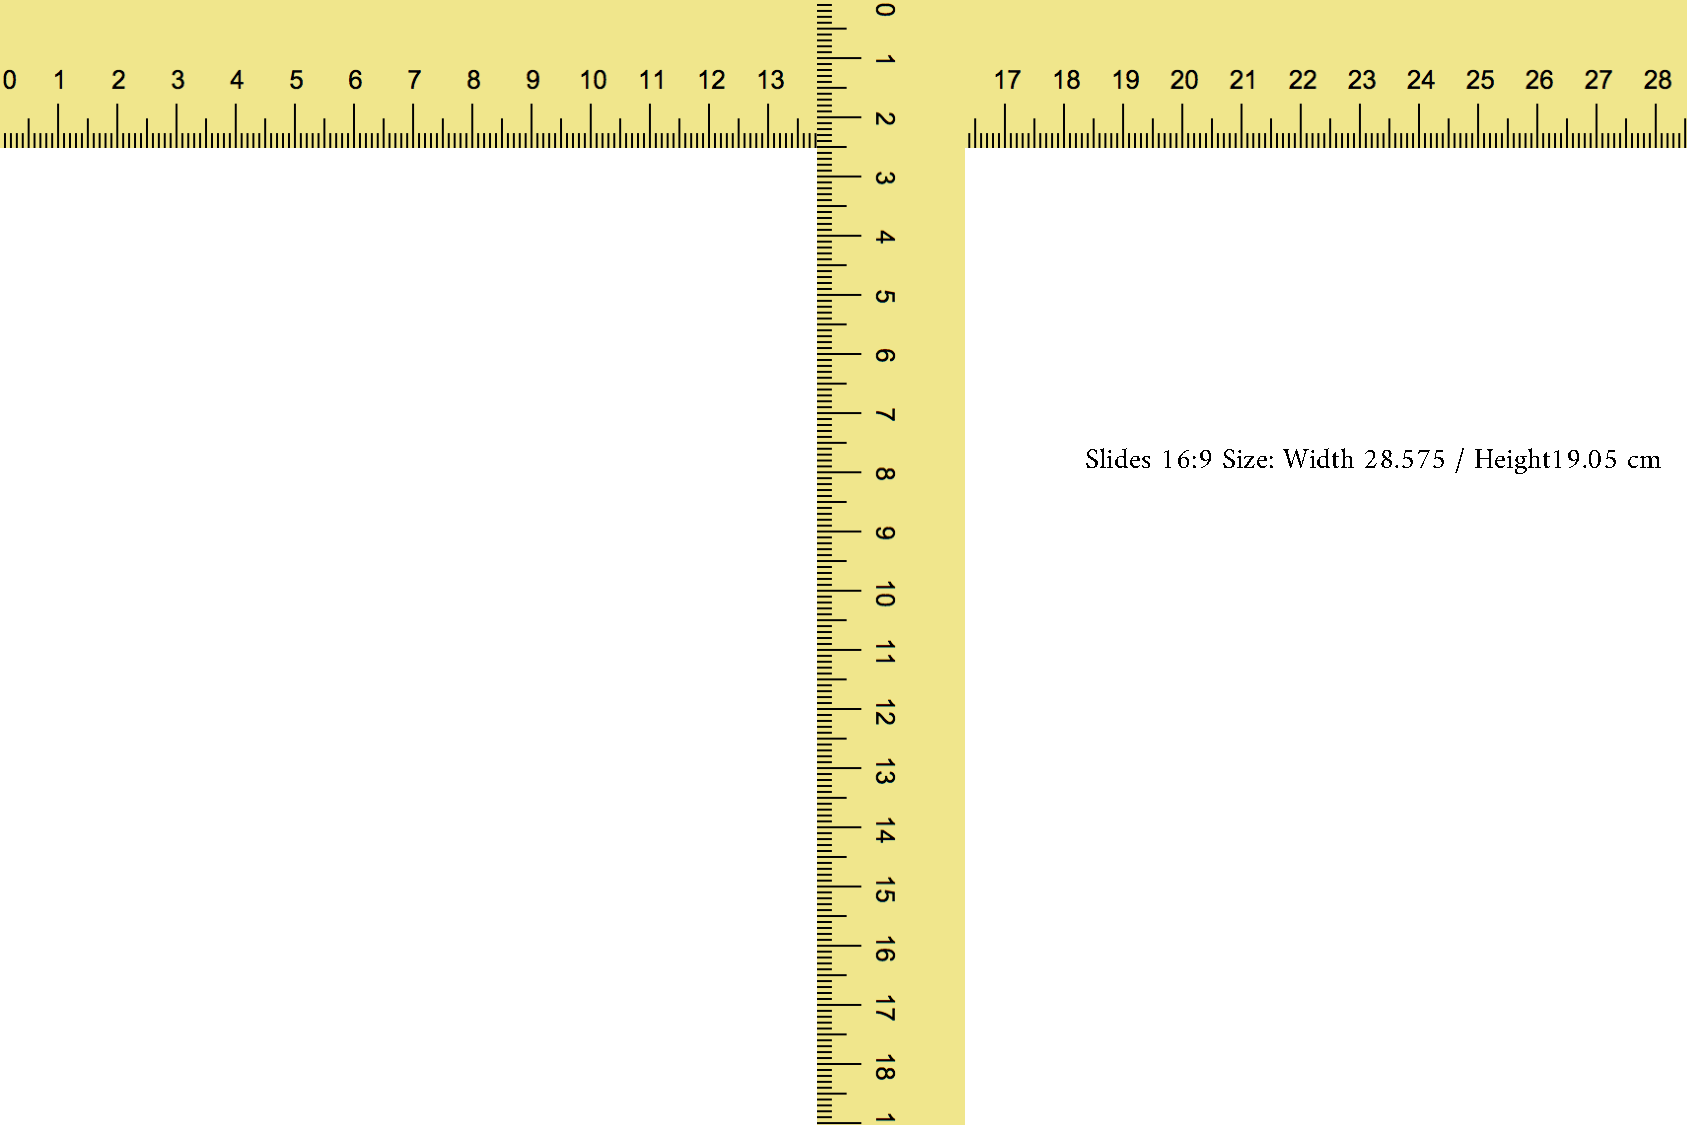
\includegraphics[width=1.\paperwidth]{Coordinates.pdf}}
\setbeamertemplate{headline}{}
\setbeamertemplate{footline}{}
\begin{frame}[t]{}
    \begin{textblock*}{0.001cm}[0.5,0.5](0.5\textwidth, 0.5\textheight)
    
\includegraphics[height = 0.25\textheight]{cat.jpeg}
    \end{textblock*}
\end{frame}
}

\subsection{Preamble}
\begin{frame}[t]{Preamble}\vspace{4pt}
\begin{itemize}
    \item Historical structures are part of the cultural heritage\vspace{10pt}\pause
    \item Stone masonry is one of the oldest construction materials\vspace{10pt}\pause
    \item Historical stone masonry structures are designed to handle gravity loads\vspace{10pt}\pause
    \item Stone masonry structure are vulnerable under seismic actions:\vspace{5pt}
    \begin{itemize}
        \item Low tensile strength
        \item Poor interlocking
        \item Large masses
        \item Built with rules-of-thumb
    \end{itemize}
\end{itemize}
\end{frame}


\breakingframe{
\begin{textblock*}{10cm}(4.7cm,2.8cm)
\Huge\textbf{\textcolor{black}{State-of-the-art}}
\end{textblock*}
\begin{textblock*}{10cm}(1.5cm,4.8cm)
\small\textbf{\textcolor{black}{{\cite{REF:5} (2018)}
}}
\end{textblock*}
}

\begin{frame}[t]{The research questions}\vspace{10pt}
    \begin{textblock*}{13cm}(1.3cm,2.8cm)
        \begin{itemize}
            \item[\textbf{Q1}] What are the expected gains of using 3D micro-mechanical modeling of stone masonry walls?\vspace{10pt}\pause
            \item[\textbf{Q2}] What tools/methods will be used to relax the 3D FE models' complexity?\vspace{20pt}\pause
            \item[\textbf{Q3}] How to estimate the stone-mortar interface strength of a simplified surfaces?
        \end{itemize}
    \end{textblock*}
\end{frame}

\breakingframe{
\begin{textblock*}{10cm}(3.7cm,2.9cm)
\Huge\textbf{\textcolor{black}{Why we are shifting to 3D micro-mechanical modeling?}}
\end{textblock*}
}


\begin{frame}[t]{Motivation: \textcolor{myviolet}{{\textbf{Q1}}}}\vspace{10pt}
    \begin{textblock*}{13cm}(1.7cm,2.7cm)
    \begin{enumerate}
        \item Stone masonry walls are usually not homogeneous through the thickness\vspace{10pt}\pause
        \item Leaf-separation effects on the strength capacity\vspace{10pt}\pause
        \item In-plane and out-of-plane behaviours interaction\vspace{10pt}\pause
        \item Internal cracking onsets and 3D crack paths (cannot be captured experimentally)
    \end{enumerate}
    \end{textblock*}
\end{frame}

\subsection{Methodology}
\begin{frame}[t]{The study main phases}\vspace{10pt}
    \begin{textblock*}{13cm}(3.8cm,0.7cm)
        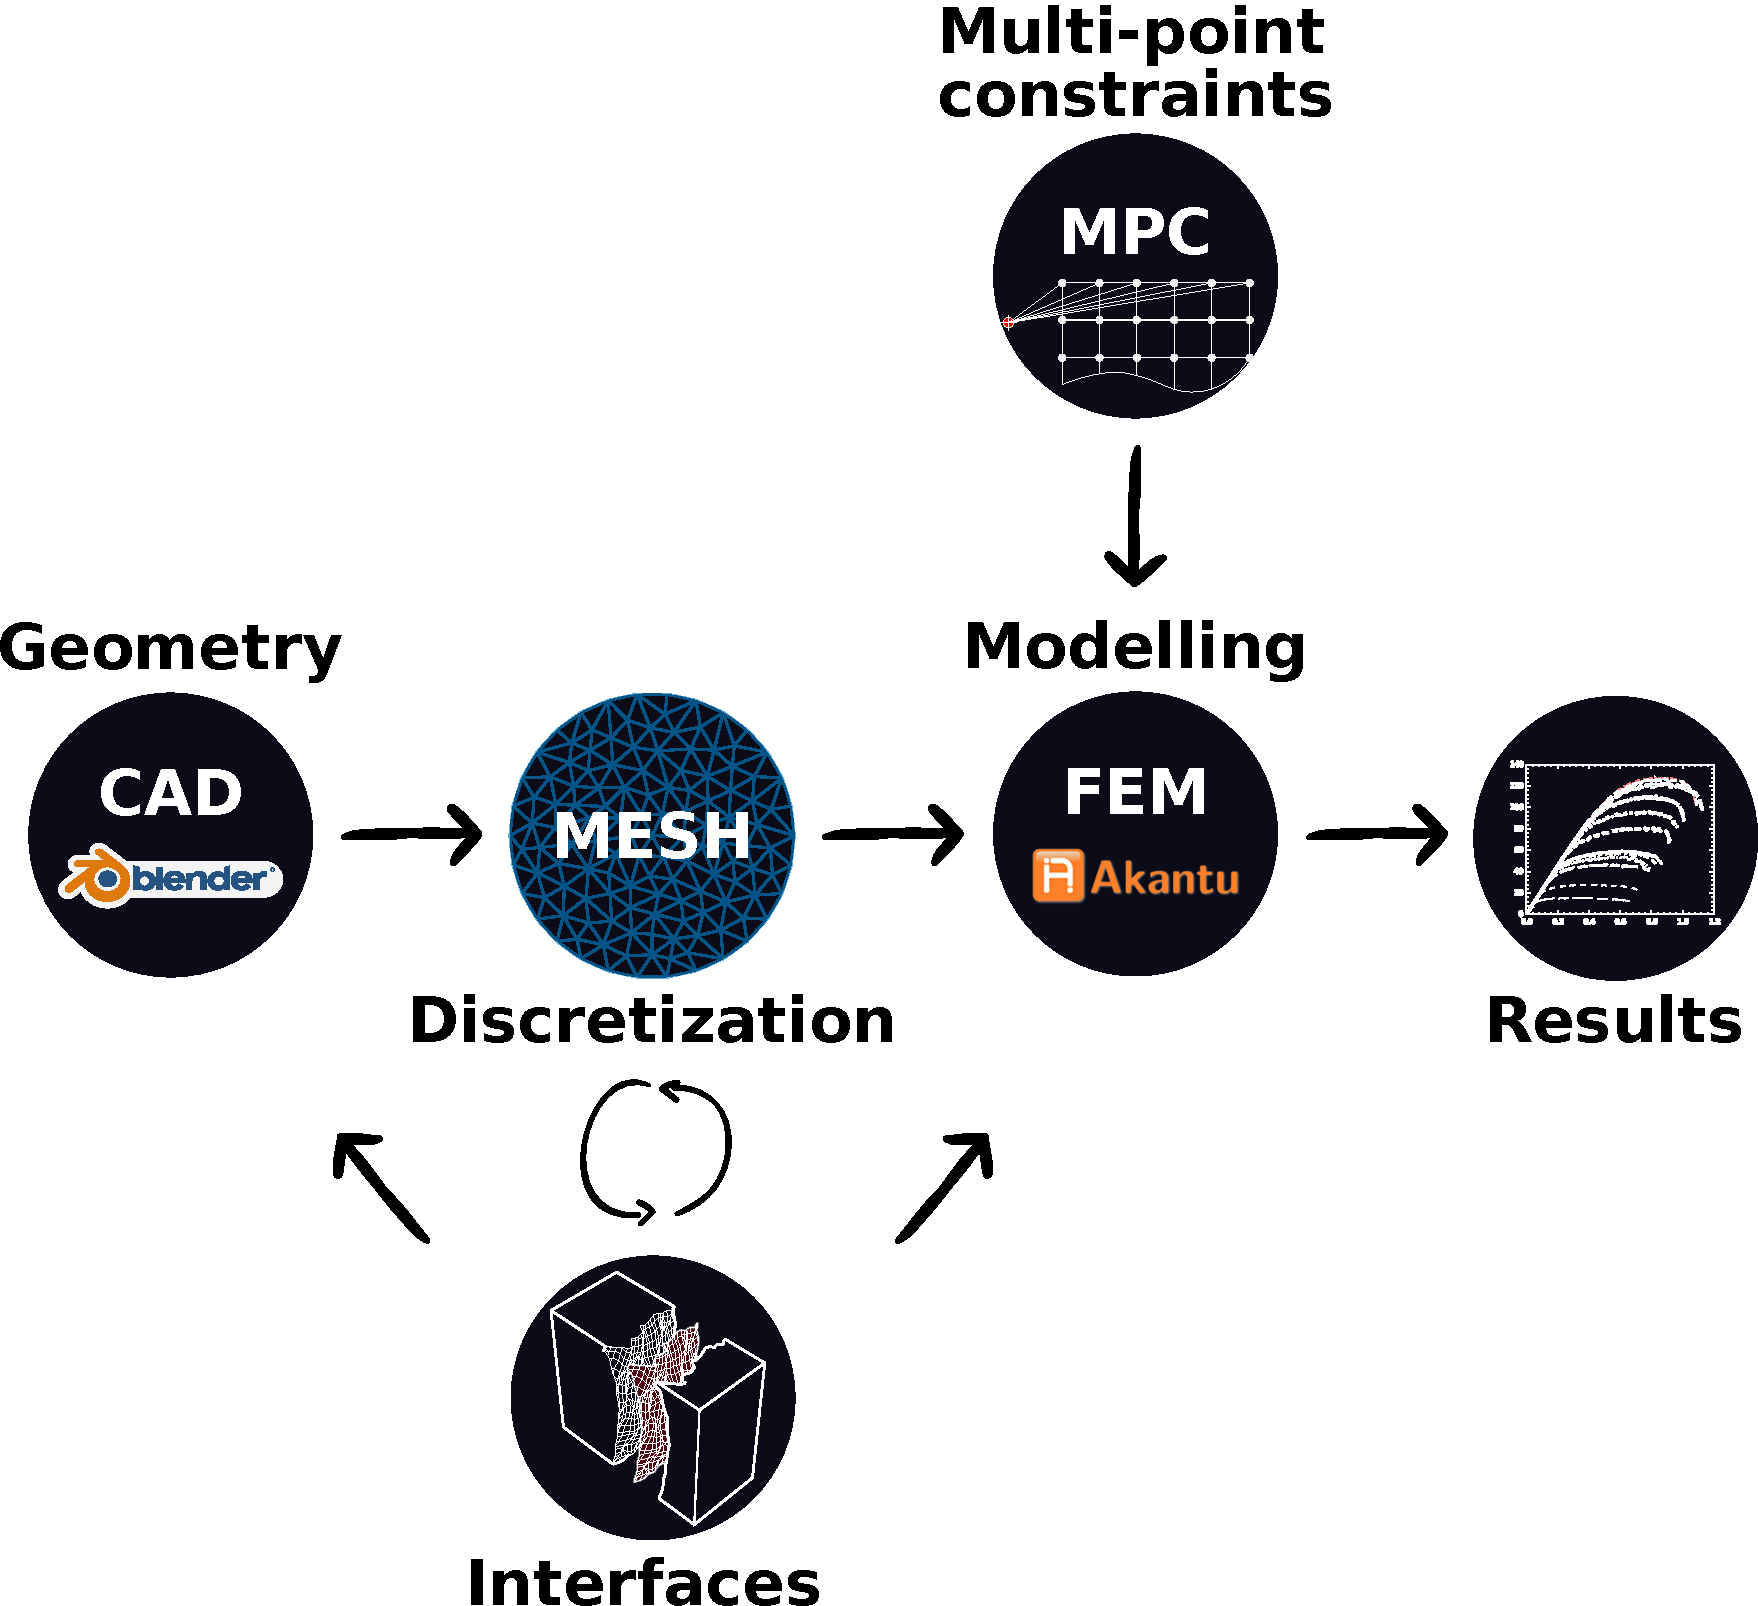
\includegraphics[height = 0.6\textwidth]{loop.pdf}
    \end{textblock*}
\end{frame}


\breakingframe{
\begin{textblock*}{13cm}(3.5cm,4cm)
\Huge\textbf{\textcolor{black}{How to arrange stones?}}
\end{textblock*}
}

\begin{frame}[t]{Objective function}\vspace{1pt}
\begin{columns}
\begin{column}{0.49\textwidth}
\begin{overprint}
\onslide<1->\begin{block}{Packing objective}
    \begin{equation*}
        \text{Minimize}~F(\vec{X_i})_{i}~=~\mid\mid \vec{S}_{i} - \vec{S}_{i-1} \mid\mid
    \end{equation*}
    \begin{equation*}
        Fitness\Big(F(\vec{X_i})\Big)_{i} = F(\vec{X_i})_{i}(1 + \xi_{1} P_A)^{\xi_{2}}
    \end{equation*}
\end{block}
\end{overprint}
\end{column}
\end{columns}
\begin{textblock*}{3.2cm}(12.5cm,1.5cm)
    \tiny{
    \begin{itemize}
        \item $S_{i}, S_{i-1}$: locations of $i$ and $i-1$ stones
        \item $\xi_{1}$: penalty multiplier
        \item $\xi_{2}$: penalty exponent
        \item $P_{A}$: penalties summation
    \end{itemize}
    }
\end{textblock*}
\begin{textblock*}{3cm}(12.5cm,1.55cm)
    
\includegraphics[height = 0.6\linewidth]{brace.pdf}
\end{textblock*}

\end{frame}


\section{Detailed plan}


\begin{frame}{Interface identification: \textcolor{myviolet}{\textbf{Q3}}}\vspace{4pt}
    \begin{textblock*}{10cm}(0.3cm, 2.5cm)
        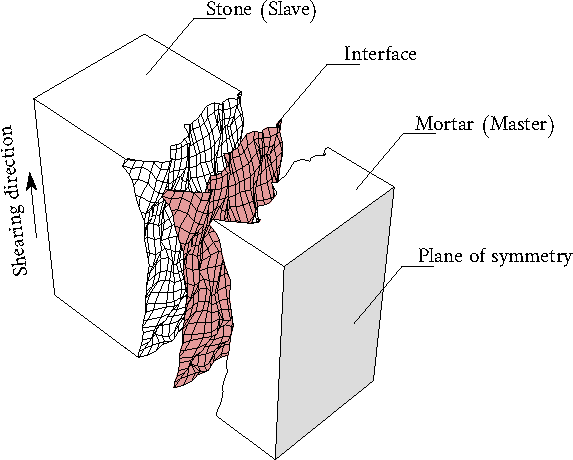
\includegraphics[height = 0.5\textwidth]{Interface.pdf}
    \end{textblock*}
    \begin{textblock*}{10cm}(6.7cm, 2.0cm)
    \begin{enumerate}
        \item Prepare real samples of stones and mortar\vspace{10pt}\pause
        \item Scan the interface surface using the laser scanner\vspace{10pt}\pause
        \item Test the samples (direct shear test)\vspace{10pt}\pause
        \item Apply different smoothing cycles on the interfaces\vspace{10pt}\pause
        \item Use the soft computing algorithms to identify the smoothed interfaces inputs (Benchmark)
    \end{enumerate}
    \end{textblock*}
\end{frame}

\begin{frame}{Call another section}
    \lipsum[5]
\end{frame}

% -----------------------References
% Thank you slide should be here
\breakingframe{
\begin{textblock*}{10cm}(3.2cm,4cm)
\Huge\textbf{\textcolor{black}{Merci de votre attention}}
\end{textblock*}
}
% -----------------------References
\section{Bibliography}
% \begin{frame}[allowframebreaks]{\\References}\vspace{4pt}
\begin{frame}{References}\vspace{4pt}
\tiny{\printbibliography}
\end{frame}
\normalsize

\end{document}